\documentclass[10pt,aspectratio=169]{beamer}

\usetheme{metropolis}
\metroset{sectionpage=none, numbering=fraction, progressbar=foot}

\usepackage[utf8]{inputenc}
\usepackage[T1]{fontenc}
\usepackage[bosnian]{babel}
\usepackage{booktabs}
\usepackage{graphicx}
\usepackage{tikz}
\usepackage{amssymb}
\usepackage{amsmath}
\usepackage{array}
\usetikzlibrary{positioning, arrows.meta, shapes.geometric}

\newcolumntype{L}[1]{>{\raggedright\arraybackslash}p{#1}}

\definecolor{accent}{HTML}{2C6E91}
\setbeamercolor{frametitle}{bg=accent}
\setbeamercolor{progress bar}{fg=accent}

\newcommand{\cmark}{\textcolor{accent}{\textbf{\checkmark}}}

\title{Voltage-Var Control (VVC) za distributivne mreže: gradient descent}
\subtitle{Seminarski rad iz predmeta SREES}
\author{Amer Muratagić}
\institute{Univerzitet u Sarajevu -- Elektrotehnički fakultet}
\date{Sarajevo, juli 2026.}

\begin{document}

{
\setbeamertemplate{footline}{}
\begin{frame}[plain]
  \titlepage
\end{frame}
}

\begin{frame}{Sadržaj}
  \setbeamertemplate{section in toc}[sections numbered]
  \tableofcontents
\end{frame}

\section{Uvod}

\begin{frame}{Motivacija i problem}
  \begin{columns}[T,onlytextwidth]
    \begin{column}{0.5\textwidth}
      \textbf{Regulacija napona nekad i sad}
      \begin{itemize}
        \item Tradicionalno: regulacioni transformatori i kondenzatorske baterije, uz pretpostavku da je tok snage dominantno usmjeren od mreže ka potrošačima.
        \item Porastom broja PV sistema ta pretpostavka više ne važi uvijek.
        \item U periodima velike proizvodnje i malog opterećenja dolazi do \textbf{obrnutog toka snage} i porasta napona u mreži.
      \end{itemize}
    \end{column}
    \begin{column}{0.5\textwidth}
      \textbf{Volt-VAR kontrola}
      \begin{itemize}
        \item Savremeni PV inverteri, osim aktivne snage $P$, mogu upravljati i reaktivnom snagom $Q$.
        \item Promjenom $Q$ utiče se na naponsko stanje mreže.
        \item Problem se posmatra kao \textbf{optimizacijski problem}: naći $Q$ za svaki PV sistem tako da naponi teže ka $1$~p.j., uz ograničenja invertera.
      \end{itemize}
    \end{column}
  \end{columns}
\end{frame}

\begin{frame}{Cilj rada}
  \textbf{Volt-VAR Descent} -- desktop aplikacija za analizu Volt-VAR kontrole u distributivnim mrežama sa PV sistemima.
  \begin{itemize}
    \item Učitavanje OpenDSS modela mreže i njegova validacija.
    \item Podešavanje parametara optimizacije i pokretanje algoritma \textbf{gradijentnog spusta}.
    \item Za svaku promjenu reaktivne snage koristi se OpenDSS rješavač toka snage (\texttt{dss\_capi}), a gradijent funkcije troška računa se numerički.
    \item Rezultati se prikazuju tekstualno (naponi, trošak, tok optimizacije) i grafički (promjena $Q$ kroz iteracije za svaki PV sistem).
  \end{itemize}
\end{frame}

\section{Alati i arhitektura}

\begin{frame}{Alati i tehnologije}
  \centering
  \small
  \begin{tabular}{L{2.6cm}L{2.4cm}L{7.5cm}}
    \toprule
    \textbf{Komponenta} & \textbf{Vrsta} & \textbf{Namjena u projektu} \\
    \midrule
    OpenDSS / \texttt{dss\_capi} & Rješavač toka snage & Učitavanje OpenDSS modela i rješavanje toka snage tokom optimizacije. \\
    natID \texttt{natGUI} & GUI okvir & Izrada grafičkog interfejsa aplikacije. \\
    natID \texttt{natPlot} & Grafički prikaz & Prikaz promjene reaktivne snage $Q$ kroz iteracije. \\
    natID \texttt{dense::DblMatrix} & Numeričke matrice & Čuvanje napona, gradijenta i historije vrijednosti $Q$. \\
    CMake & Sistem izgradnje & Konfiguracija projekta i povezivanje biblioteka. \\
    \bottomrule
  \end{tabular}
\end{frame}

\begin{frame}[fragile]{Arhitektura aplikacije}
  \begin{columns}[T,onlytextwidth]
    \begin{column}{0.48\textwidth}
      \textbf{Struktura projekta}
      {\scriptsize
      \begin{semiverbatim}
VoltVarDescent/
|-- CMakeLists.txt
|-- examples/   (primjeri feedera)
`-- src/
    |-- main.cpp
    |-- MainWindow.h
    |-- DSSEngine.h
    |-- network/  (Network tab)
    `-- solver/   (Solver tab)
      \end{semiverbatim}
      }
    \end{column}
    \begin{column}{0.52\textwidth}
      \textbf{Klasa \texttt{DSSEngine}}
      \begin{itemize}
        \item Jedina veza aplikacije sa OpenDSS API-jem -- GUI ne poznaje detalje \texttt{dss\_capi}.
        \item Sadrži metodu \texttt{runVanillaGD}, gdje je implementiran cijeli optimizacijski dio: podešavanje PV sistema, tok snage, funkcija troška, gradijent i historija.
      \end{itemize}
    \end{column}
  \end{columns}
\end{frame}

\section{Gradient descent algoritam}

\begin{frame}{Algoritam \texttt{runVanillaGD}}
  \begin{columns}[T,onlytextwidth]
    \begin{column}{0.55\textwidth}
      \begin{enumerate}
        \small
        \item Svi PV sistemi se postave na $Q=0$; izračunaju se početni naponi i početni trošak.
        \item Za svaki PV sistem: pomjeri se $Q$ za $+\varepsilon$ i $-\varepsilon$, riješi se tok snage i dobiju $C^+$, $C^-$.
        \item Gradijent po komponenti $j$ procjenjuje se centralnom razlikom:
        \[
          g_j \approx \frac{C^+ - C^-}{2\varepsilon}
        \]
        \item Reaktivne snage se ažuriraju u smjeru smanjenja troška, uz ograničenje koraka $\Delta_{\max}$.
        \item Ponovo se rješava tok snage i bilježi stanje u historiju.
      \end{enumerate}
    \end{column}
    \begin{column}{0.45\textwidth}
      \textbf{Kriterij zaustavljanja}
      \footnotesize
      \begin{itemize}
        \item najveća promjena $Q$ manja od tolerancije, ili
        \item dostignut maksimalan broj iteracija.
      \end{itemize}
      \vspace{0.6em}
      \textbf{Parametri solvera}
      \footnotesize
      \begin{itemize}
        \item max. broj iteracija, brzina učenja
        \item max. korak $Q$, korak $\varepsilon$
        \item granica reaktivne snage, tolerancija
      \end{itemize}
    \end{column}
  \end{columns}
\end{frame}

\section{Grafički interfejs}

\begin{frame}{Network tab}
  \begin{columns}[c,onlytextwidth]
    \begin{column}{0.42\textwidth}
      \centering
      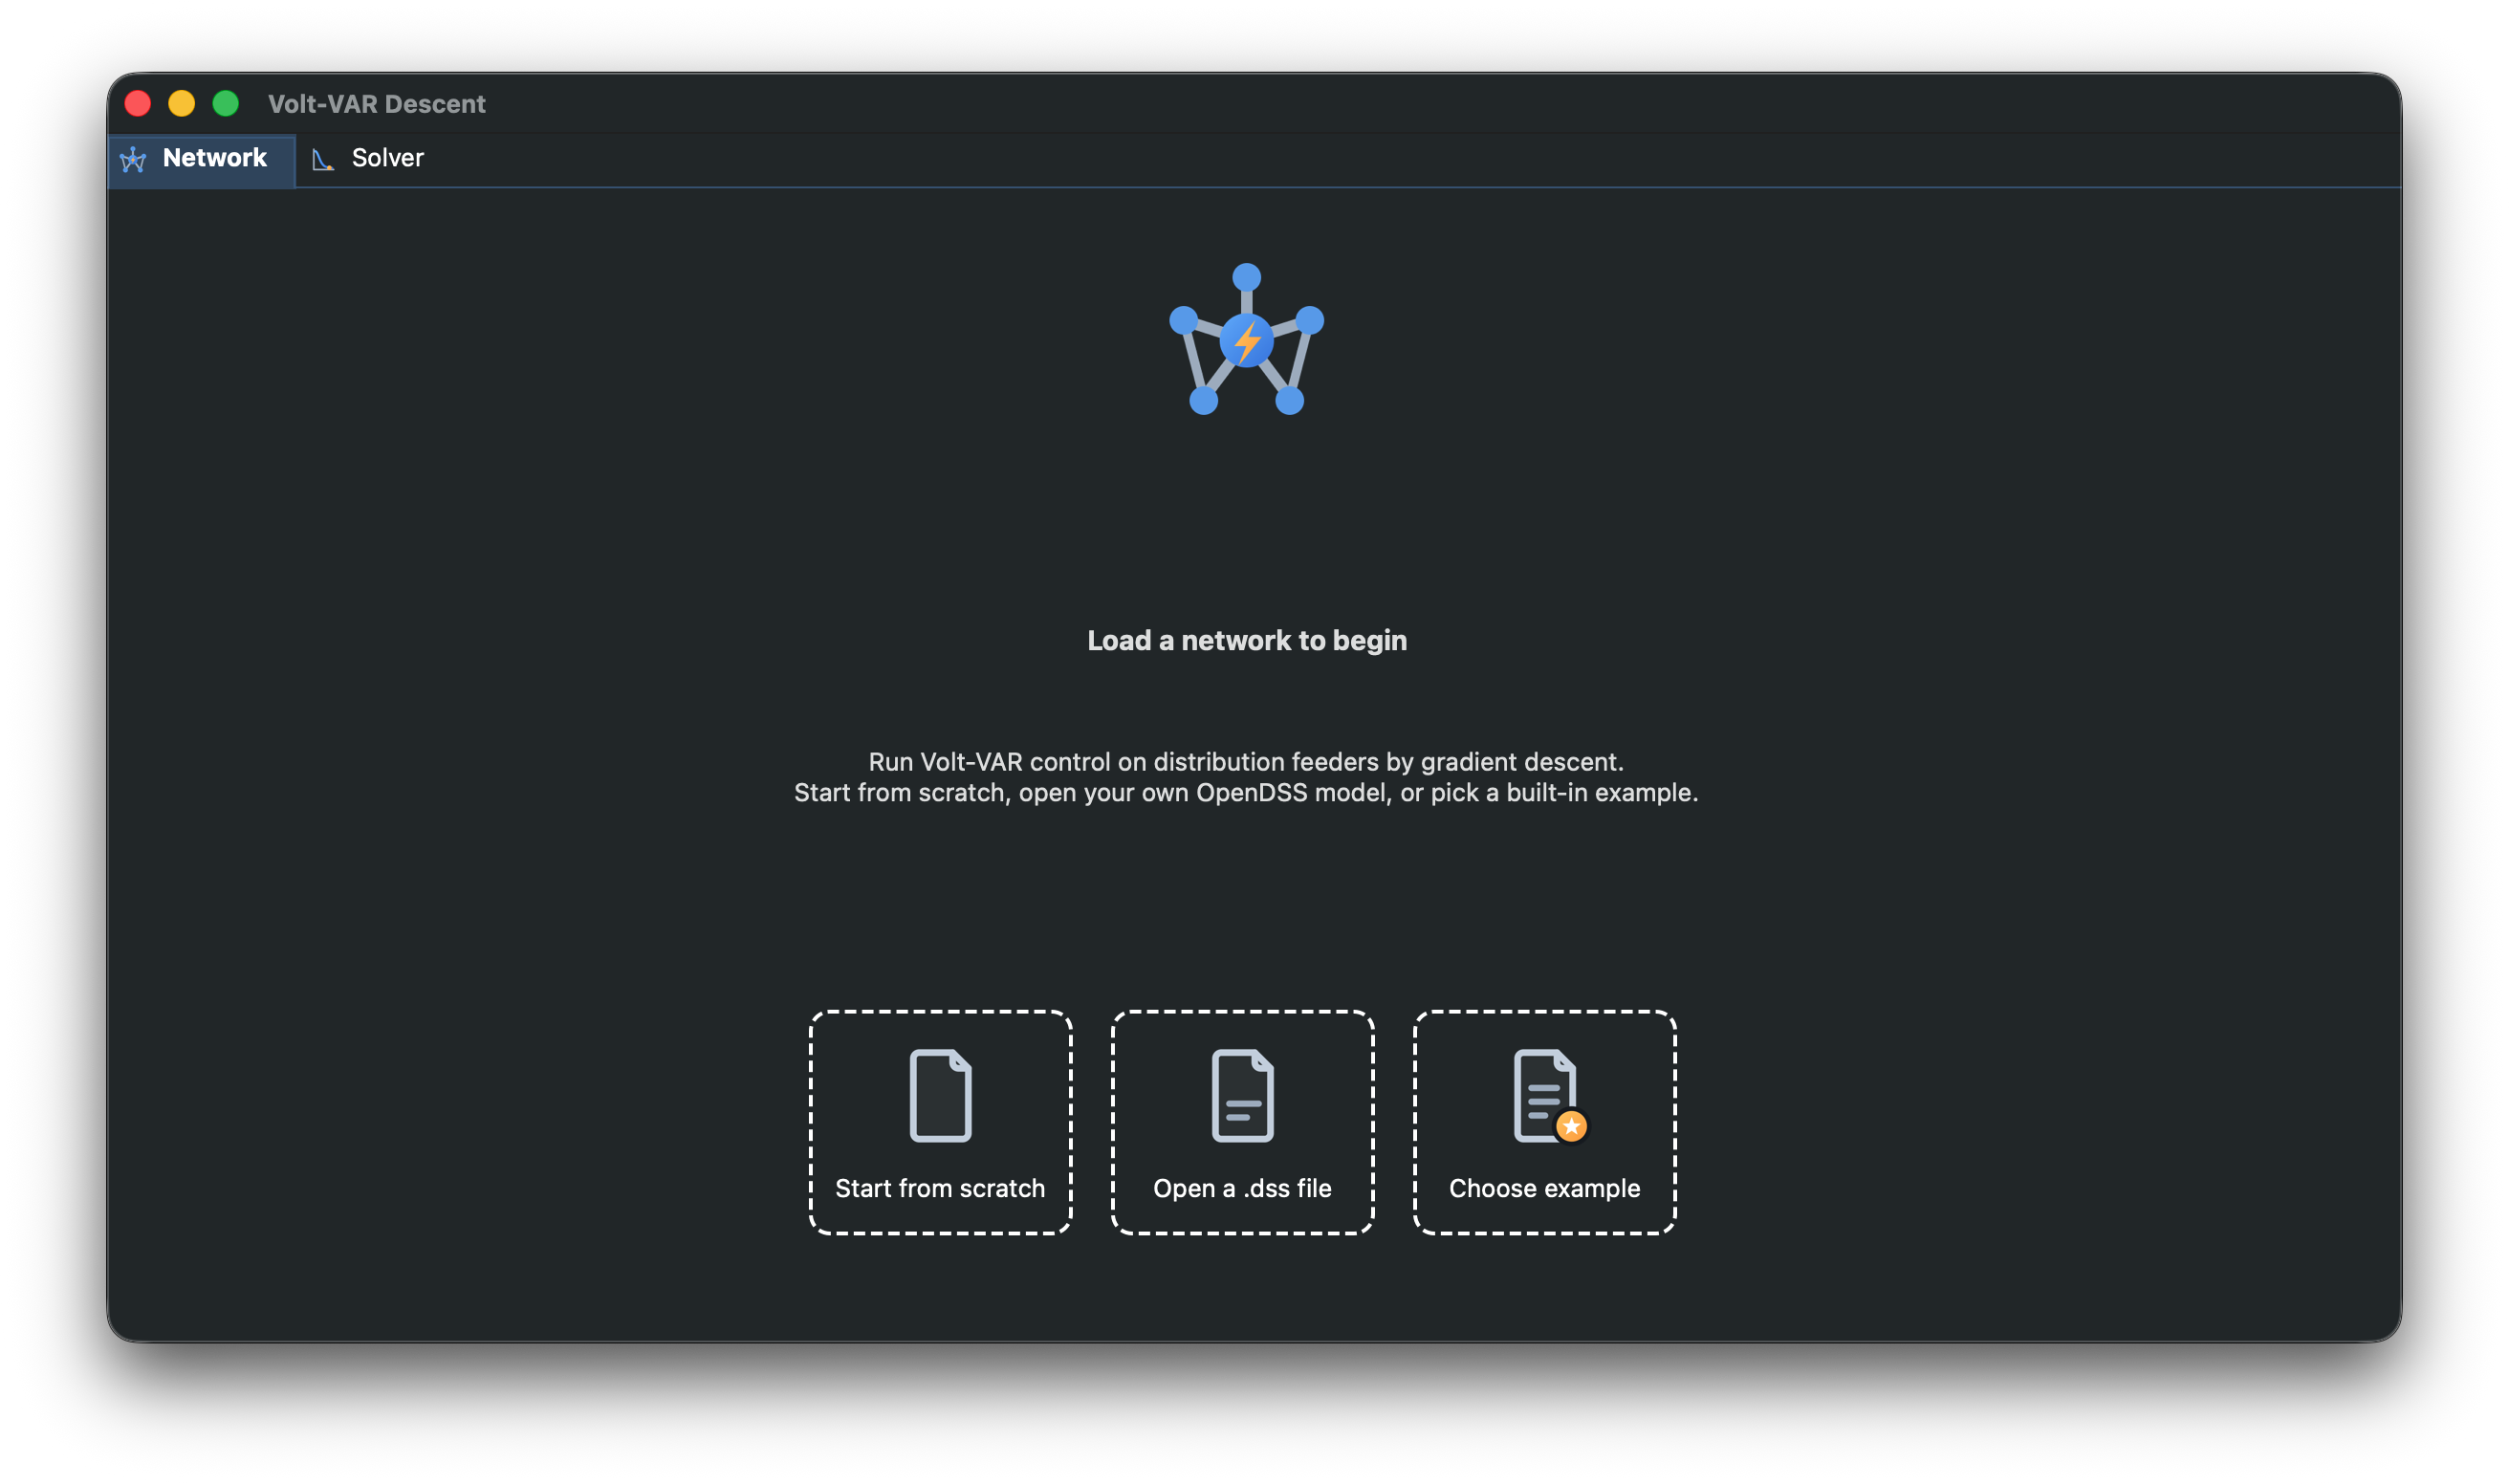
\includegraphics[width=0.95\textwidth]{assets/network_tab.png}\\
      \footnotesize Početni ekran -- prazan editor, otvaranje \texttt{.dss} datoteke ili ugrađeni primjer
    \end{column}
    \begin{column}{0.58\textwidth}
      \centering
      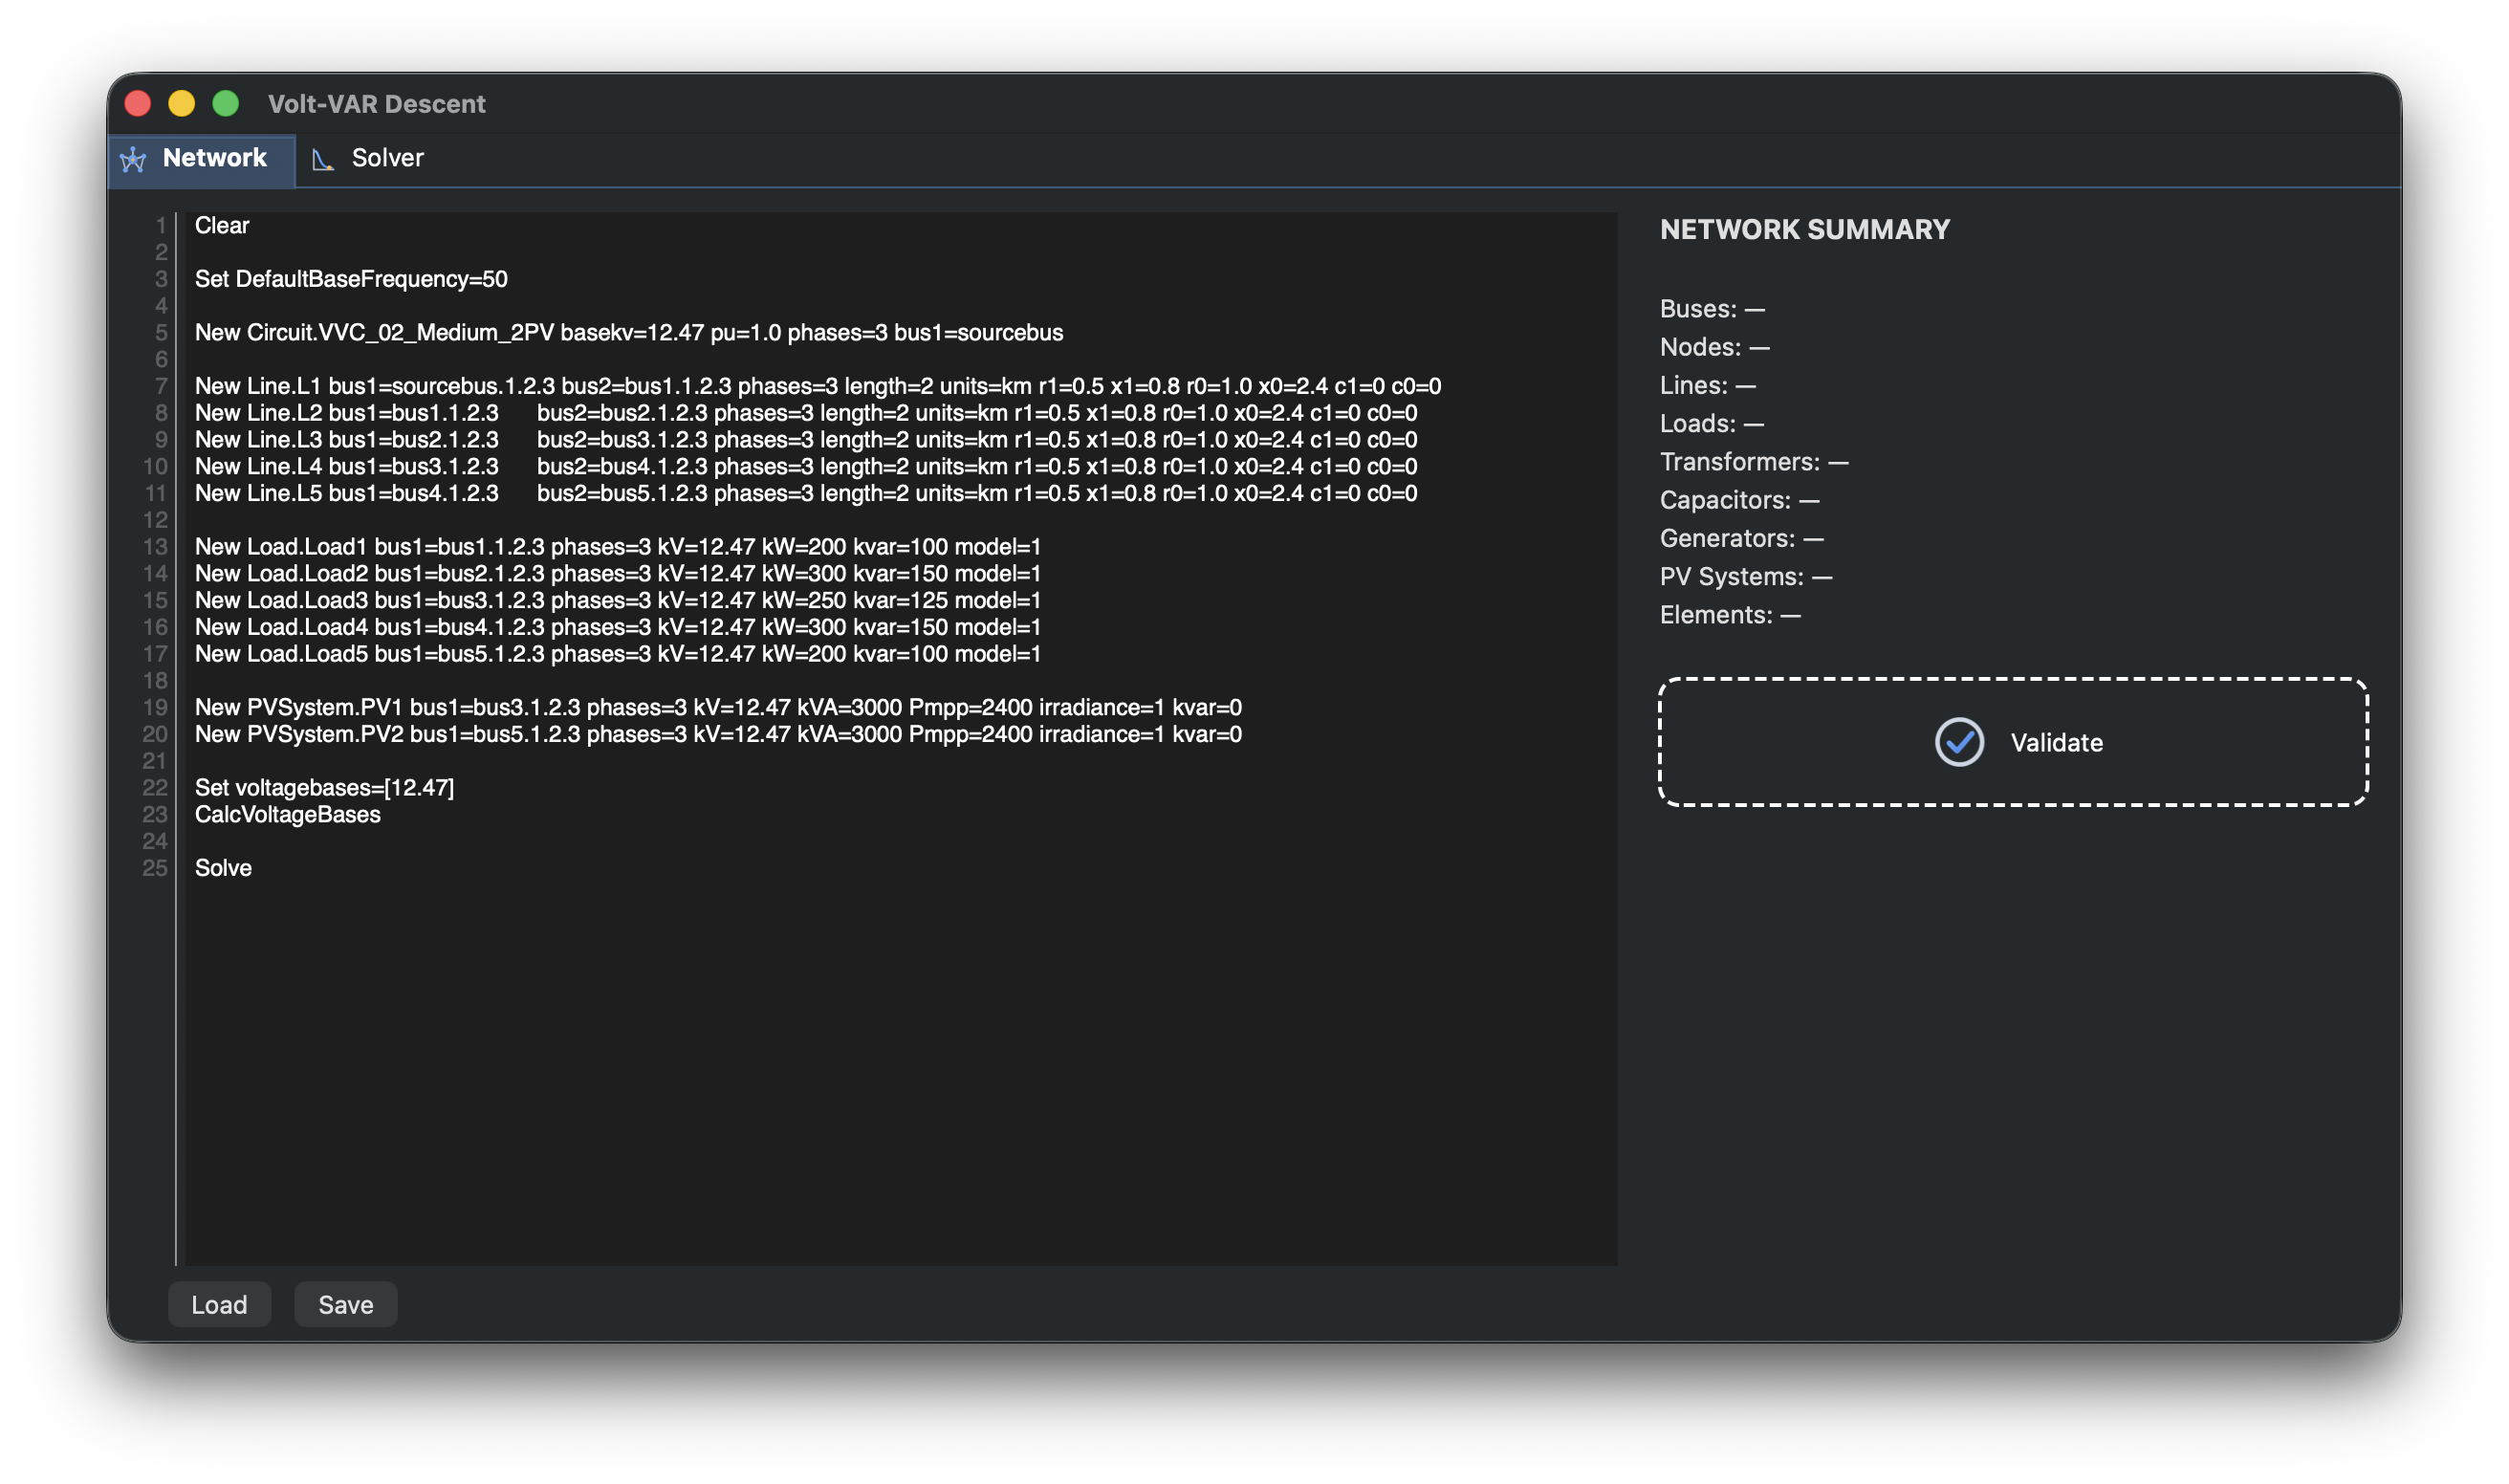
\includegraphics[width=0.95\textwidth]{assets/network_tab_editor.png}\\
      \footnotesize Editor OpenDSS skripte i sažetak mreže nakon validacije
    \end{column}
  \end{columns}
  \vspace{0.4em}
  \footnotesize Validacija je obavezna prije pokretanja solvera; svaka izmjena skripte poništava validaciju i zaključava \textit{Solver} tab.
\end{frame}

\begin{frame}{Solver tab}
  \begin{columns}[c,onlytextwidth]
    \begin{column}{0.5\textwidth}
      \centering
      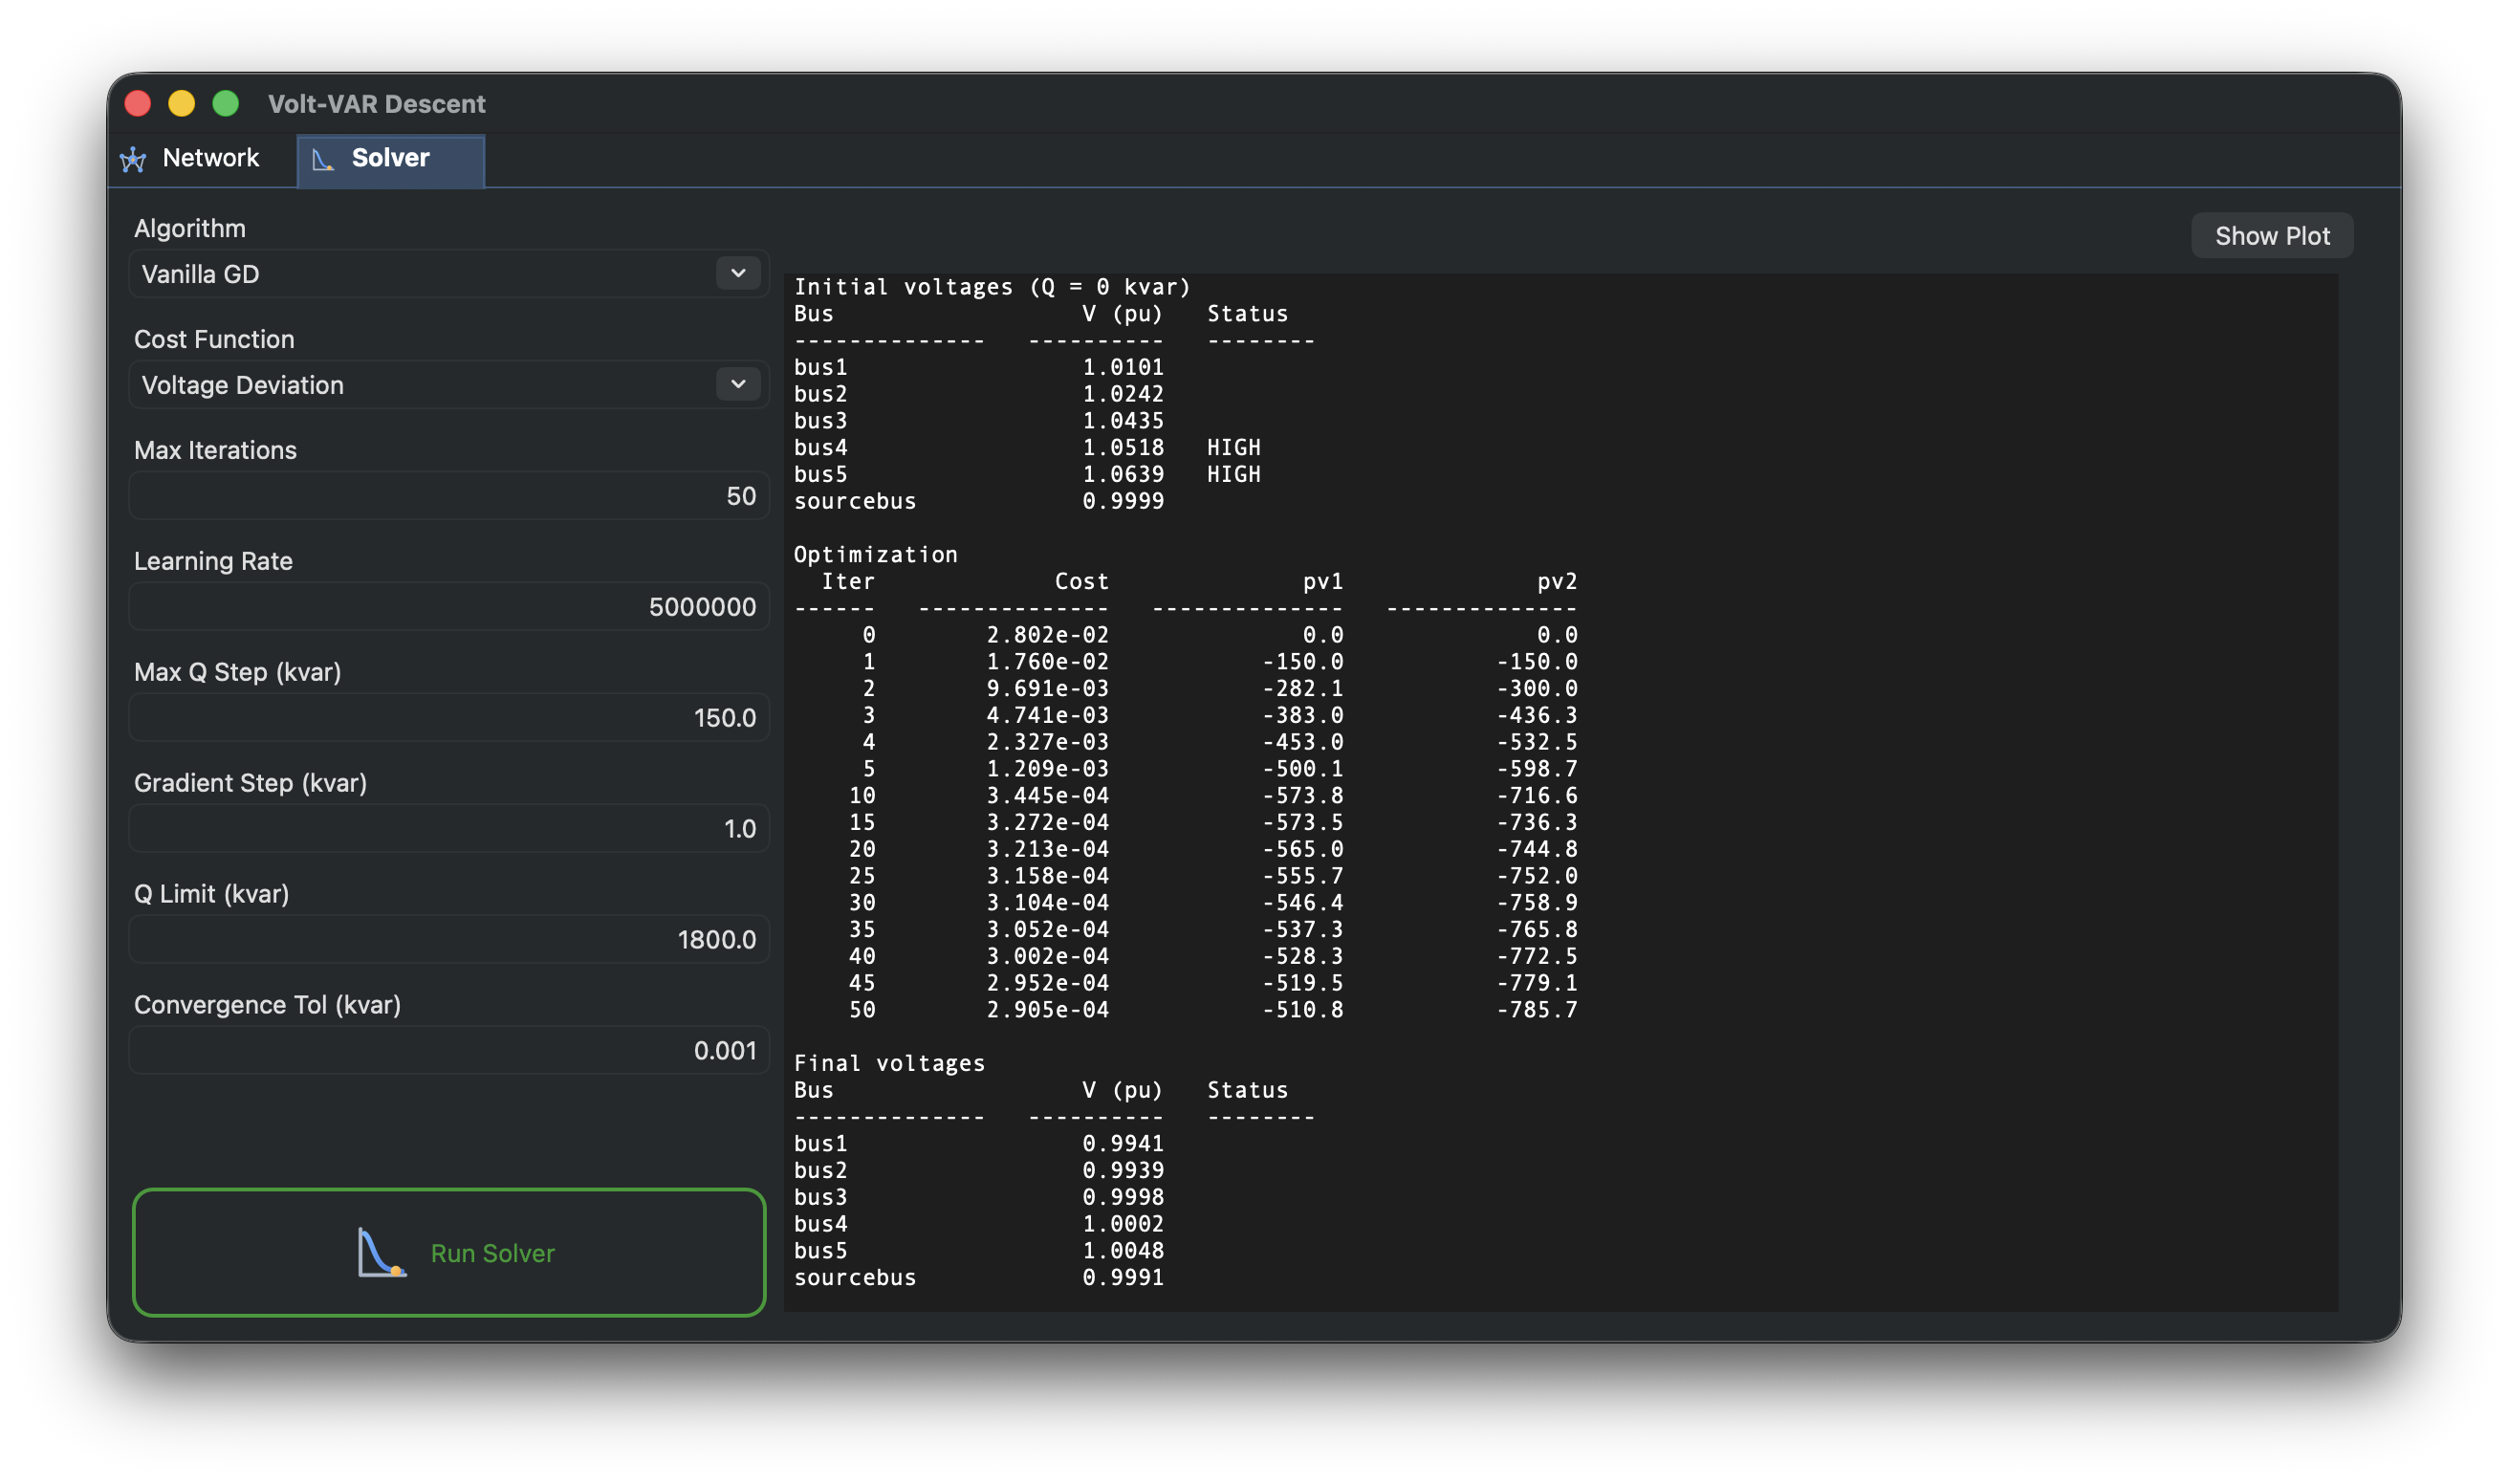
\includegraphics[width=0.95\textwidth]{assets/solver_text.png}\\
      \footnotesize Tekstualni prikaz -- početni/konačni naponi i tok optimizacije po iteracijama
    \end{column}
    \begin{column}{0.5\textwidth}
      \centering
      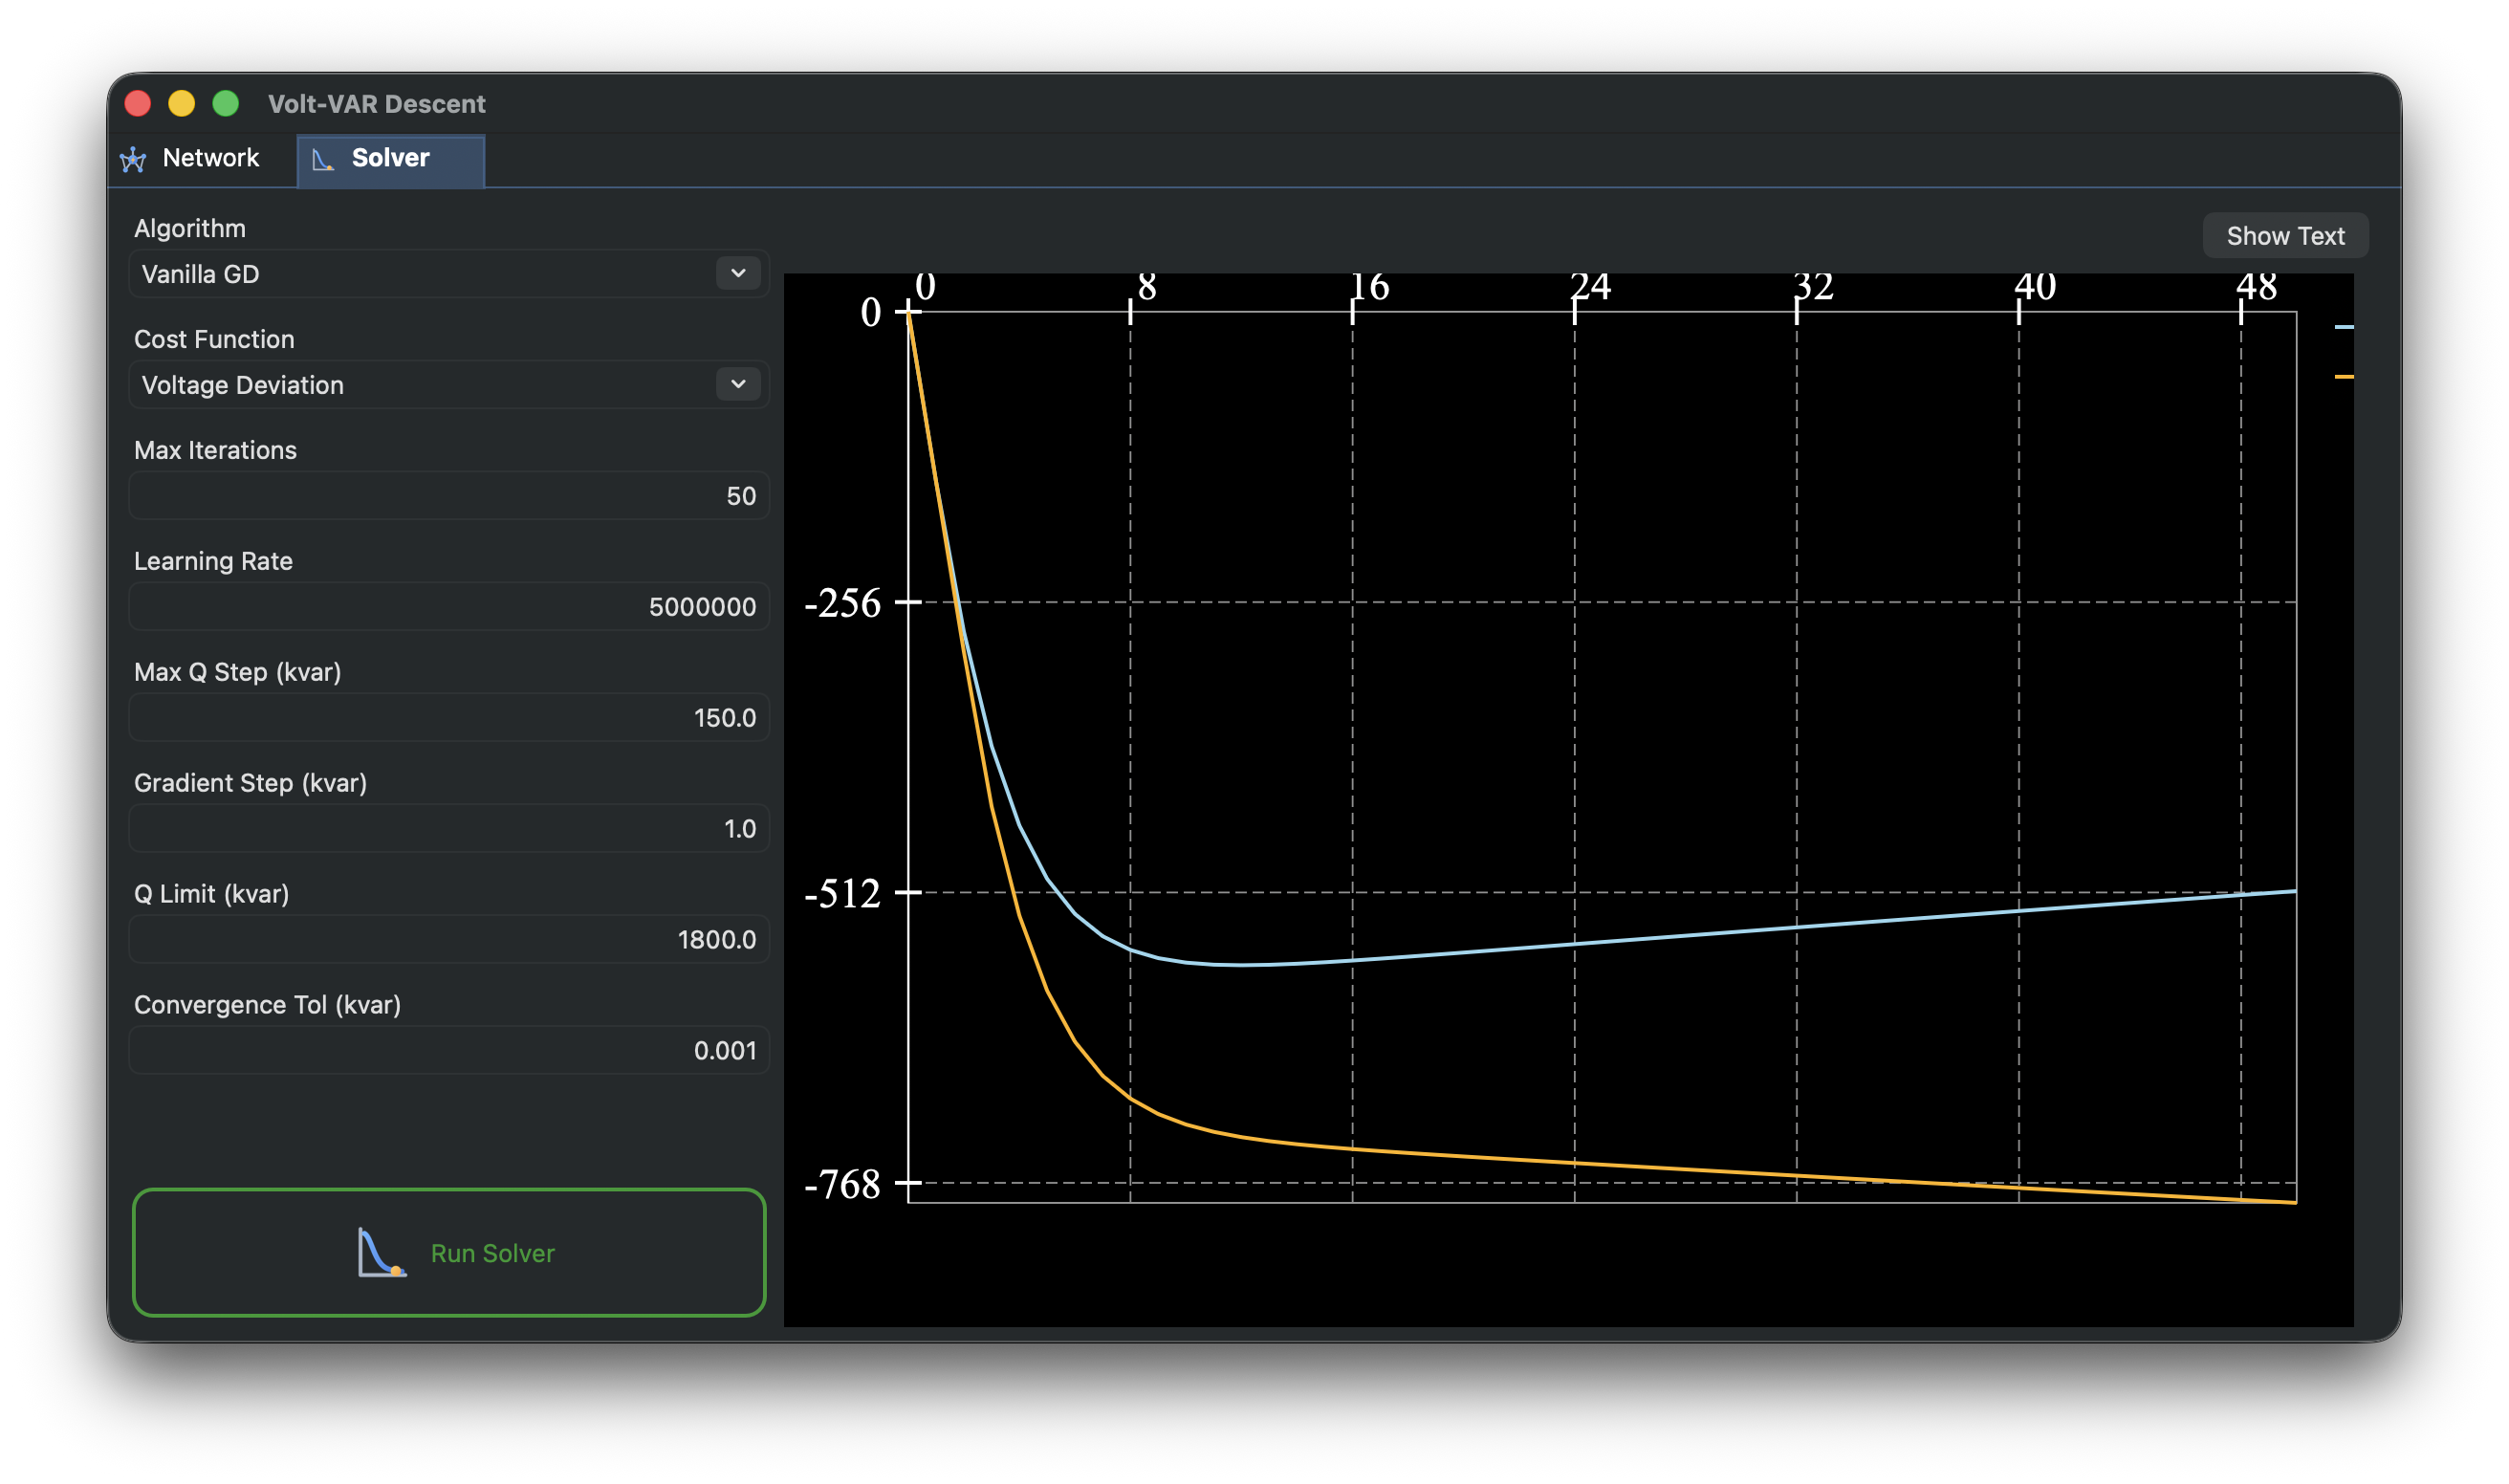
\includegraphics[width=0.95\textwidth]{assets/solver_plot.png}\\
      \footnotesize Grafički prikaz -- promjena $Q$ za svaki PV sistem kroz iteracije
    \end{column}
  \end{columns}
  \vspace{0.4em}
  \footnotesize Dostupno tek nakon uspješne validacije mreže
\end{frame}

\section{Zaključak}

\begin{frame}{Zaključak}
  \begin{itemize}
    \item Implementirana je C++ desktop aplikacija \textbf{Volt-VAR Descent} za Volt-VAR kontrolu u mrežama sa PV sistemima.
    \item Tokove snaga rješava OpenDSS preko \texttt{dss\_capi}; gradijent funkcije troška računa se numerički (centralna razlika).
    \item Pristup je jednostavan za implementaciju i radi nad proizvoljnim OpenDSS modelom, ali zahtijeva više rješavanja tokova snage po iteraciji.
  \end{itemize}
  \vspace{0.3em}
  \textbf{Mogući nastavak:} dodatne funkcije troška, druge varijante gradijentnog spusta, testiranje na složenijim mrežama.

\end{frame}

{
\setbeamertemplate{footline}{}
\begin{frame}[standout]
  Hvala na pažnji!\\[0.3em]
  \vspace{1em}
\end{frame}
}

\end{document}
